\documentclass[letterpaper,11pt]{article}
\oddsidemargin -1.0cm \textwidth 17.5cm

\usepackage[utf8]{inputenc}
\usepackage[activeacute,spanish, es-lcroman]{babel}
\decimalpoint
\usepackage{amsfonts,setspace}
\usepackage{amsmath}
\usepackage{amssymb, amsmath, amsthm}
\usepackage{comment}
\usepackage{float}
\usepackage{amssymb}
\usepackage{dsfont}
\usepackage{anysize}
\usepackage{multicol}
\usepackage{enumerate}
\usepackage{graphicx}
\usepackage[left=1.5cm,top=2cm,right=1.5cm, bottom=1.7cm]{geometry}
\setlength\headheight{1.5em} 
\usepackage{fancyhdr}
\usepackage{multicol}
\usepackage{hyperref}
\usepackage{wrapfig}
\usepackage{subcaption}
\usepackage{siunitx}
\usepackage{cancel}
\usepackage{mdwlist}
\usepackage{svg}
\pagestyle{fancy}
\fancyhf{}
\renewcommand{\labelenumi}{\normalsize\bfseries P\arabic{enumi}.}
\renewcommand{\labelenumii}{\normalsize\bfseries (\alph{enumii})}
\renewcommand{\labelenumiii}{\normalsize\bfseries \roman{enumiii})}


\begin{document}

\fancyhead[L]{\itshape{Facultad de Ciencias F\'isicas y Matem\'aticas}}
\fancyhead[R]{\itshape{Universidad de Chile}}
\rfoot[]{pág. \thepage}

\begin{minipage}{11.5cm}
    \begin{flushleft}
        \hspace*{-0.6cm}\textbf{FI1100 Introducción a la Física Moderna}\\
        \hspace*{-0.6cm}\textbf{Tutor:} Alejandro Cartes
    \end{flushleft}
\end{minipage}

\begin{picture}(2,3)
    \put(366, -10){
\includegraphics[scale=0.9]{Imágenes/logo/dfi-fcfm.pdf}}
\end{picture}

\begin{center}
	\LARGE\textbf{Tutoría C1}\\
	\Large{MAS y Ondas}
\end{center}

\vspace{-1cm}
\begin{enumerate}\setlength{\itemsep}{0.4cm}

\item[]

\item Un cuerpo de masa $m$ se encuentra restringido a moverse en una circunferencia de radio $R$. Esta masa además se encuentra atada a un resorte de constante elástica $k$ y largo natural $\ell_0$.

\begin{multicols}{2}
\begin{enumerate}
    \item Determine la posición de equilibrio

    \item Encuentre la ecuación de movimiento de la masa $m$ para pequeñas oscilaciones
    
    \item[]
\end{enumerate}
\columnbreak

\begin{figure}[H]
    \centering
    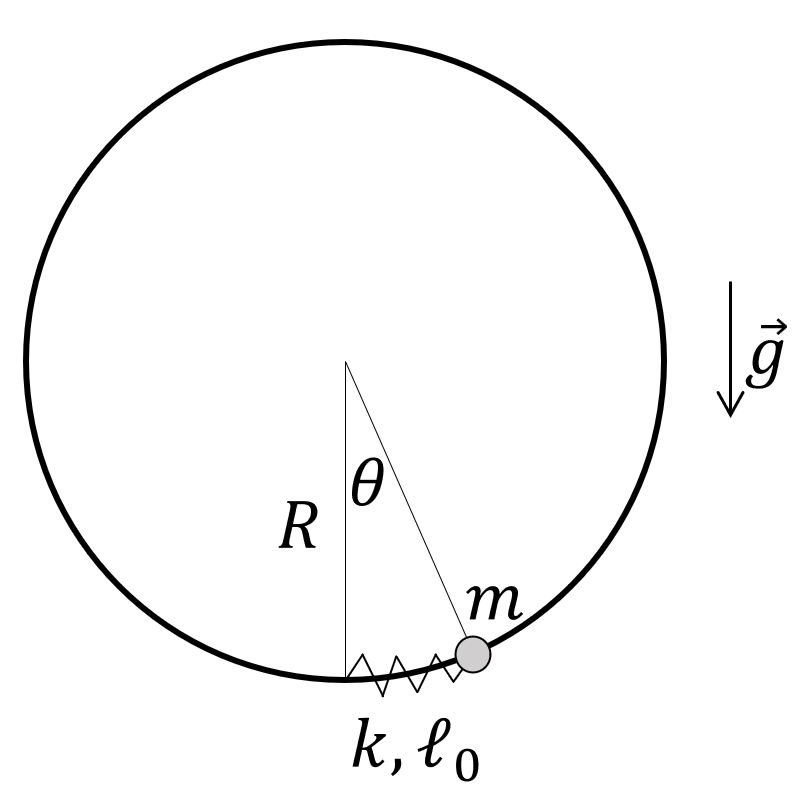
\includegraphics[width=0.38\linewidth]{Imágenes/tutorias/resorte-circ.png}
\end{figure}
\end{multicols}


\item
\begin{multicols}{2}
    Se suelta un péndulo de masa $m$ desde el reposo, de modo tal que desciende y choca elásticamente con un bloque de igual masa. Encuentre la ecuación de movimiento del bloque tras la colisión, considerando que en $t=0$ los resortes están en su largo natural $\ell_0$. Ignore la presencia del péndulo después del choque

    \columnbreak

    \begin{figure}[H]
        \centering
        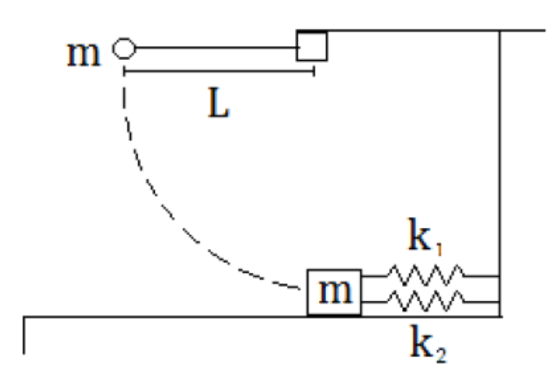
\includegraphics[width=0.5\linewidth]{Imágenes/tutorias/pendulo-resorte.png}
    \end{figure}
\end{multicols}

\item Considere una cuerda ideal, muy larga, en posición horizontal. La tensión de la cuerda es $T$ y su densidad lineal de masa $\mu$. En el instante inicial, se genera un pulso que viaja hacia la derecha cuya forma está dada por la función $f(x)$ y otro que viaja hacia la izquierda, cuya forma está determinada por la función $g(x)$. Las funciones correspondientes son:
\begin{align*}
    f(x) &= \exp{[-(x+x_0)^2]} & g(x) &= \exp{[-(x-x_0)^2]}
\end{align*}

\begin{enumerate}
    \item Dibuje la forma de la cuerda en el tiempo inicial $t=0$. Suponga que $x_0$ lo suficientemente grande

    \item Determine el tiempo $t^*$ en que ambos pulsos se encuentran. Dibuje la forma de la cuerda en ese instante

    \item Determine una expresión analítica para la velocidad transversal de la cuerda. ¿Qué ocurre con esta en $t^*$?
\end{enumerate}

% \item Dos cuerdas de densidad lineal de masa $R$ y $2R$ se unen entre sí, con la cuerda de mayor densidad en el lado derecho. Los extremos de la cuerda están unidos a masas $M$. Se dispone de dos pivotes, separados a una distancia $2L$, sobre los cuales posa la cuerda en forma horizontal como se indica en la figura. En un cierto instante se generan dos pulsos idénticos y simétricos en cada uno de los extremos de la cuerda. Determine la distancia, medida desde el extremo izquierdo de la cuerda, donde se encuentran los puntos centrales de ambos pulsos.

\item
\begin{enumerate}
    \item Demuestre que $y(x,t) = 4x^2 + 9 t^2 + 12xt + 12x + 18t + 30$ es solución de la ecuación de ondas. ¿En qué dirección avanza la onda?

    \item Demuestre que $y(x,t) = \sin{x}\cos{(vt)}$ es solución de la ecuación de ondas y que puede escribirse de la forma $y(x,t) = f(x-vt)+g(x+vt)$
\end{enumerate}


% Para imágenes vectoriales -> el texto tiene que estar en LaTeX
% \begin{figure}[htbp]
%   \centering
%   \svgpath{../Imagenes/ejercicios}  -> .. irse pa'trás 
%   \includesvg{ej5.svg}
% \end{figure}

\end{enumerate}
\end{document}
